\documentclass[11pt]{article}
\usepackage[a4paper,margin=2.2cm]{geometry}
\usepackage[T1]{fontenc}
\usepackage[utf8]{inputenc}
\usepackage{lmodern}
\usepackage{hyperref}
\usepackage{graphicx}
\usepackage{float}
\usepackage{booktabs}
\usepackage{longtable}
\usepackage{array}
\usepackage{enumitem}
\usepackage{xcolor}
\usepackage{fancyhdr}
\usepackage{titlesec}
\hypersetup{colorlinks=true,linkcolor=black,urlcolor=blue,citecolor=black}
\setlength{\parindent}{2em}
\setlength{\parskip}{0.35em}
\renewcommand{\arraystretch}{1.25}
\pagestyle{fancy}
\fancyhf{}
\fancyhead[L]{VICOO-ESP User Document Draft}
\fancyhead[R]{\thepage}
\titleformat{\section}{\Large\bfseries}{\thesection}{0.6em}{}
\titleformat{\subsection}{\large\bfseries}{\thesubsection}{0.6em}{}
\newcommand{\projectname}{VICOO-ESP}
% 本文件位于仓库 \texttt{tex/}；配图在同目录 \texttt{user-manual-figures/}。默认用 Playwright 截 \texttt{http://vicoo.yhazrin.xyz/} 与 \texttt{/impact/shop/2}（见 \texttt{playwright.manual-figures.config.ts}）；U3 仍为本地 admin。
%   \texttt{cd frontend/web-react \&\& npm run screenshots:manual}
% 编译请在 \texttt{tex/} 下执行 \texttt{pdflatex "7\_user\_draft (2).tex"}，或将整个 \texttt{tex/} 上传 Overleaf。
\newcommand{\placeholder}[1]{\begin{figure}[H]\centering\fbox{\parbox[c][4.2cm][c]{0.86\linewidth}{\centering #1}}\end{figure}}
\begin{document}

\begin{center}
{\LARGE \textbf{Group 7\_user\_draft}}\\[0.5em]
{\large \projectname{} User Document (Draft)}\\[0.5em]
Usage Guide for System Testing\\
\end{center}

\section*{Document Purpose}
This document explains how different user groups are expected to use the \projectname{} system and provides a practical basis for system testing. It is aligned with the current repository layout: a \textbf{React (Vite)} consumer site (\texttt{frontend/web-react}), a separate \textbf{admin console} (\texttt{admin}), and a \textbf{FastAPI} back end (\texttt{backend}).

The draft is organised into three chapters: \textbf{consumer users}, \textbf{internal staff / administrators}, and \textbf{partners / supply chain information providers}. The partner chapter describes a \emph{roadmap} capability: the current codebase does not expose a dedicated partner login portal; partner names may appear as fields inside supply-chain records on the consumer timeline. If course rules require only implemented roles, omit or shorten that chapter while keeping the overall structure.

During testing, the following principles are recommended:
\begin{enumerate}[leftmargin=2.2em]
    \item validate complete user journeys rather than testing isolated buttons only;
    \item check not only whether a page opens, but also whether information is displayed correctly and data stays consistent across shop, detail page, and admin views;
    \item if content was drafted with AI assistance, verify that the final displayed version has been manually reviewed and revised;
    \item fill in the final testing URLs, accounts, and screenshots before submission.
\end{enumerate}

\tableofcontents

\section{System Overview and Preparation}
\subsection{System Overview}
\projectname{} is a web-based system centred on sustainable fashion, product traceability, and charity-oriented storytelling. The consumer application offers \textbf{two storefronts}:
\begin{itemize}[leftmargin=2.2em]
    \item \textbf{Company shop} --- route prefix \texttt{/shop} (standard catalogue experience).
    \item \textbf{Impact shop} --- route prefix \texttt{/impact/shop} (charity / impact-oriented catalogue; full-screen \textbf{Traceability Globe} is shown only for eligible products; see \S\ref{sec:globe}).
\end{itemize}
On a product detail page, users can read narrative copy, sustainability score, optional linked artwork, and a \textbf{supply-chain timeline} fed by the API. When the immersive globe is active, the timeline stays linked to the selected node. Internal staff use the admin console to manage orders, campaigns, artworks, donations, users, products (including impact flags and trace narrative fields), and audit-related views. Supply-chain \emph{stage} rows (nodes) consumed by the globe/timeline are provided by the back-end API; they are not edited on the current \texttt{Products} admin screen, so testers should confirm journey data via the deployment process (e.g.\ database seed or API) used in your environment.

\subsection{Recommended Environment}
To ensure stable interaction and WebGL globe performance, the following environment is recommended:
\begin{enumerate}[leftmargin=2.2em]
    \item desktop browser: recent versions of Chrome, Edge, or Safari;
    \item recommended resolution: no lower than 1440 $\times$ 900;
    \item network environment: stable campus or home broadband connection;
    \item for admin upload workflows, desktop use is recommended.
\end{enumerate}

\subsection{Login and Account Preparation}
\textbf{Consumers} can browse public catalogue pages without an account. The current consumer app \textbf{blocks checkout until login} (logged-out visitors to \texttt{/checkout} see a login prompt). \textbf{Product reviews} and \textbf{profile} also require authentication. The \texttt{/orders/:id} page calls the orders API; whether a guest can open another user's order depends on server-side authorization---test both allowed and denied cases in your environment.

\textbf{Staff} sign in to the admin application (separate origin/port from the consumer site in local development).

\textbf{Partners:} no standalone partner portal is shipped in the current tree; skip partner credentials unless you add such a feature.

The final testing version should fill in:
\begin{itemize}[leftmargin=2.2em]
    \item consumer site base URL: \texttt{[to be filled]} (e.g.\ \texttt{http://localhost:9111} in dev);
    \item admin console URL: \texttt{[to be filled]};
    \item test consumer account (for reviews/checkout): \texttt{[to be filled]};
    \item test staff account: \texttt{[to be filled]}.
\end{itemize}

\section{Consumer User Guide}
\subsection{User Goal}
The main goal of a consumer user is to browse products, understand sustainability and traceability context, and complete support or purchase steps where enabled. The system emphasises a \emph{discover -- understand -- verify} journey: catalogue $\rightarrow$ detail $\rightarrow$ timeline/globe (when available) $\rightarrow$ optional cart and post-purchase views.

\subsection{Main Functions}
Consumer users can access the following (route names refer to the consumer app):
\begin{enumerate}[leftmargin=2.2em]
    \item browse \texttt{/shop} or \texttt{/impact/shop};
    \item open \texttt{/shop/:id} or \texttt{/impact/shop/:id} for product detail;
    \item read images, description, trace story, sustainability score, and optional linked artwork;
    \item interact with the \textbf{Traceability Globe} when the product and route satisfy the conditions in \S\ref{sec:globe};
    \item read the \textbf{timeline} synced with globe selection (and scroll behaviour as implemented);
    \item inspect per-stage fields on the timeline when present (e.g.\ partner name, verification flag, carbon notes);
    \item use \textbf{cart} and \textbf{checkout} (\texttt{/checkout}) where enabled;
    \item open \textbf{order detail} (\texttt{/orders/:id}) after purchase;
    \item submit \textbf{reviews} on the detail page when logged in;
    \item open the \textbf{AI assistant} (\texttt{/assistant}) from the product page shortcut when testing conversational help.
\end{enumerate}

\subsection{Typical Flow 1: From Shop to Product Detail}
\textbf{Steps:}
\begin{enumerate}[leftmargin=2.2em]
    \item Open the homepage or go directly to \texttt{/shop} or \texttt{/impact/shop}.
    \item Browse product cards (title, thumbnail, summary).
    \item Click a card to open the matching detail URL (\texttt{/shop/:id} or \texttt{/impact/shop/:id}).
    \item Confirm that copy, price, media, and impact-specific blocks render without blank critical sections.
\end{enumerate}

\textbf{Expected result:}
The detail page loads; navigation back to the correct shop (\texttt{/shop} vs \texttt{/impact/shop}) works. Layout is readable and consistent with the design system.

\IfFileExists{user-manual-figures/u1-homepage.png}{%
\begin{figure}[H]\centering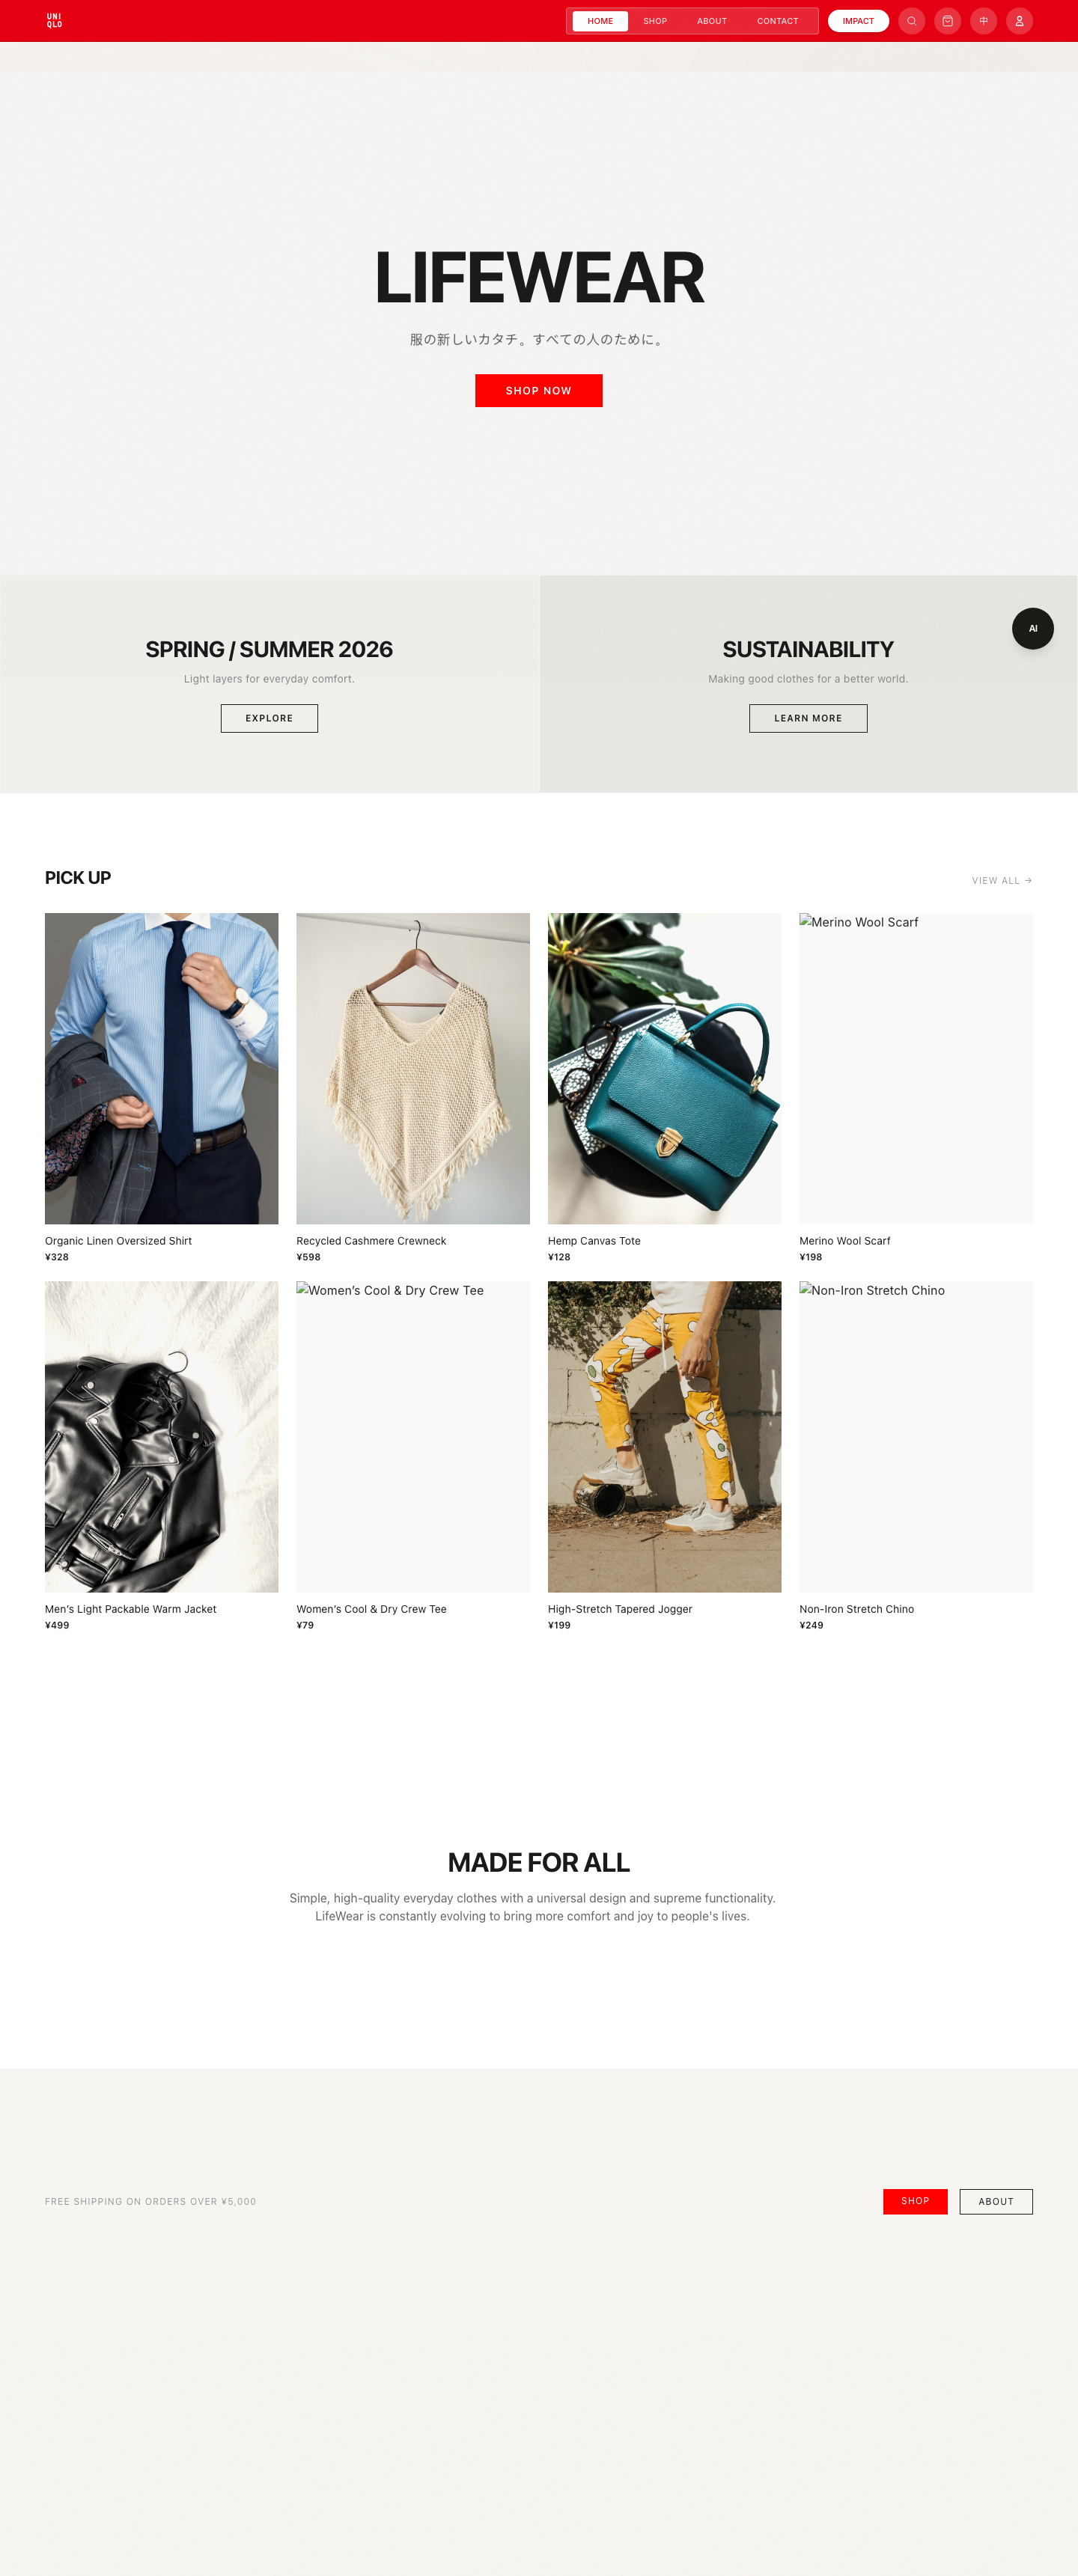
\includegraphics[width=0.94\linewidth]{user-manual-figures/u1-homepage.png}\caption*{Figure U1: Site homepage (\texttt{http://vicoo.yhazrin.xyz/}).}\end{figure}%
}{\placeholder{Generate \texttt{user-manual-figures/u1-homepage.png} via \texttt{npm run screenshots:manual}.}}

\subsection{Typical Flow 2: Traceability Globe (Impact Products)}
\label{sec:globe}
\textbf{Preconditions (current implementation):} The immersive, full-viewport globe appears on the detail page only when \textbf{all} hold: the product is marked as an impact product, the URL is under \texttt{/impact/shop/:id}, and the product has at least one supply-chain timeline record from the API. Otherwise, testers should still see the timeline section where data exists, but not the full-screen globe layout.

\textbf{Steps:}
\begin{enumerate}[leftmargin=2.2em]
    \item Open an impact product detail URL that satisfies the preconditions.
    \item Locate the globe and confirm nodes render at expected geographic positions.
    \item Click nodes; confirm the detail panel or linked timeline reflects the same stage.
    \item Switch between nodes; confirm no stale labels or mismatched media.
\end{enumerate}

\textbf{Expected result:}
Nodes respond to input; selected stage information matches API data. If WebGL fails, note browser, GPU, and console errors.

\IfFileExists{user-manual-figures/u2-globe-timeline.png}{%
\begin{figure}[H]\centering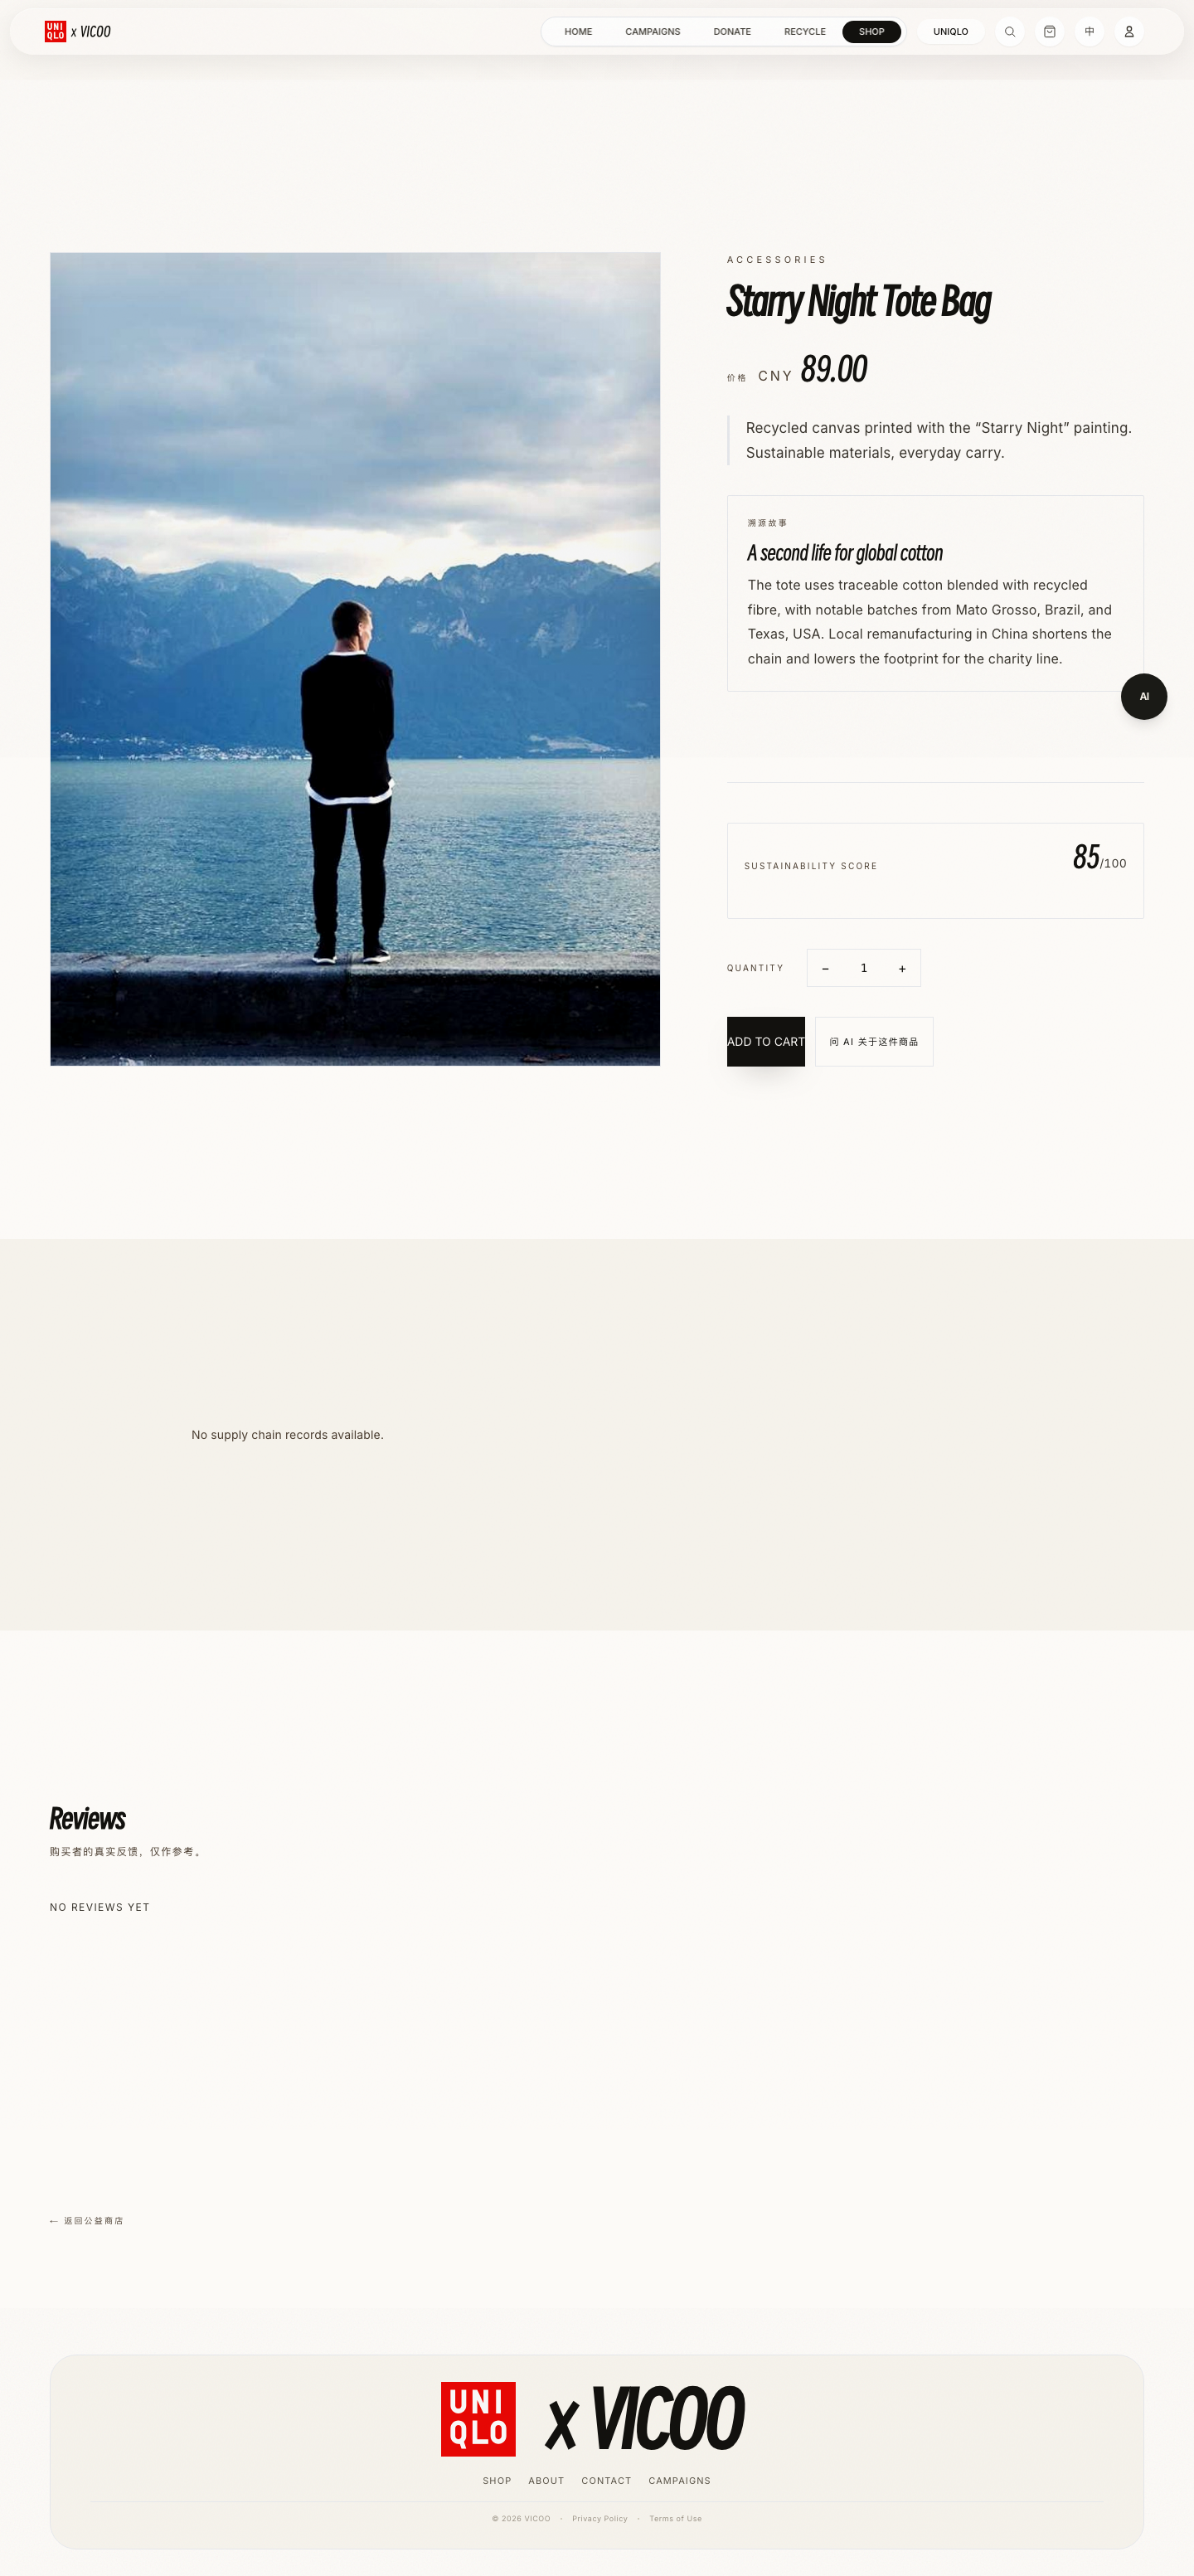
\includegraphics[width=0.94\linewidth]{user-manual-figures/u2-globe-timeline.png}\caption*{Figure U2: Traceability globe and timeline (\texttt{/impact/shop/2}).}\end{figure}%
}{\placeholder{Generate \texttt{user-manual-figures/u2-globe-timeline.png} via \texttt{npm run screenshots:manual}.}}

\subsection{Typical Flow 3: Timeline and Scroll Behaviour}
\textbf{Steps:}
\begin{enumerate}[leftmargin=2.2em]
    \item On a detail page with timeline data, scroll through the page.
    \item Observe highlight or focus changes on timeline entries relative to scroll or globe selection.
    \item If click-to-focus is implemented, select a timeline row and confirm the globe selection updates.
\end{enumerate}

\textbf{Expected result:}
The user can follow the supply-chain story in order; linkage between globe and timeline remains consistent with the latest selection.

\subsection{Typical Flow 4: Stage-Level Verification and Environmental Notes}
\textbf{Steps:}
\begin{enumerate}[leftmargin=2.2em]
    \item Expand or focus individual timeline stages.
    \item When the API provides them, read verification flags, partner labels, carbon mass (\texttt{carbon\_kg}), and free-text carbon notes.
\end{enumerate}

\textbf{Expected result:}
Numeric and textual fields are human-readable and consistent with back-end data. There is \textbf{no} separate ``global search'' or standalone ``carbon comparison dashboard'' route in the consumer \texttt{App.tsx}; do not file defects for absent modules that are out of scope.

\subsection{Typical Flow 5: Cart and Checkout}
\textbf{Steps:}
\begin{enumerate}[leftmargin=2.2em]
    \item From a detail page, add an in-stock item to the cart (cart drawer).
    \item Open \texttt{/checkout} and complete the flow supported by your deployment.
    \item Open \texttt{/orders/:id} for the created order when an ID is available.
\end{enumerate}

\textbf{Expected result:}
Totals, status, and identifiers match server responses; errors are surfaced clearly.

\subsection{Typical Flow 6: Reviews (Authenticated)}
\textbf{Steps:}
\begin{enumerate}[leftmargin=2.2em]
    \item Register or log in via \texttt{/register} or \texttt{/login}.
    \item Open a product detail page; scroll to the reviews section.
    \item Submit a rating and text; confirm the new review appears after refresh according to API behaviour.
\end{enumerate}

\textbf{Expected result:}
Guests see existing reviews but not the submission form; authenticated users can post subject to validation.

\subsection{Typical Flow 7: AI Assistant Entry Point}
\textbf{Steps:}
\begin{enumerate}[leftmargin=2.2em]
    \item From a product detail page, use the shortcut to \texttt{/assistant} (product context may be passed in navigation state).
    \item Ask a product-related question and verify answers respect visible catalogue facts.
\end{enumerate}

\textbf{Expected result:}
The assistant loads; responses are safe to quote only after human review for any public-facing demo.

\subsection{Common Questions for Consumer Users}
\textbf{Question 1: Why do some nodes contain less information than others?}\\
Answer: Data completeness depends on back-end records. Each important stage should at least identify the stage; empty stages indicate incomplete seeding or API data.

\textbf{Question 2: Why is there no globe on my product?}\\
Answer: Check that you used \texttt{/impact/shop/:id}, that the product is an impact product, and that journey data exists. Standard \texttt{/shop/:id} items may show a simpler timeline block only.

\textbf{Question 3: The globe is slow or freezes. What should I do?}\\
Answer: Try hardware acceleration, update the browser, close heavy tabs, and retest. Record GPU/OS for the defect report.

\section{Internal Staff / Administrator Guide}
\subsection{User Goal}
Staff maintain operational and editorial data that powers the consumer site: catalogue, campaigns, charitable flows, orders, compliance-related audits, and user records. Accuracy, auditability, and alignment with front-end routes (\texttt{/shop} vs \texttt{/impact/shop}) matter more than visual polish alone.

\subsection{Roles and Permissions}
The FastAPI user model includes roles such as \texttt{admin}, \texttt{editor}, \texttt{user}, \texttt{guardian}, and \texttt{compliance}. The admin SPA may further distinguish UI labels (e.g.\ viewer/auditor in local types). Tests should document which role each account holds and verify least-privilege behaviour for your deployment.

\subsection{Main Functions (Admin Console Navigation)}
After login, the sidebar exposes (paths from \texttt{admin/src/App.tsx}):
\begin{enumerate}[leftmargin=2.2em]
    \item \textbf{Dashboard} --- \texttt{/}
    \item \textbf{Artworks} --- \texttt{/artworks}
    \item \textbf{Campaigns} --- \texttt{/campaigns}
    \item \textbf{Donations} --- \texttt{/donations}
    \item \textbf{Orders} --- \texttt{/orders}
    \item \textbf{Clothing donations} --- \texttt{/clothing-donations}
    \item \textbf{After-sales} --- \texttt{/after-sales}
    \item \textbf{Users} --- \texttt{/users}
    \item \textbf{Products} --- \texttt{/products}
    \item \textbf{Child audit} --- \texttt{/child-audit}
    \item \textbf{Settings} --- \texttt{/settings}
    \item \textbf{Audit log} --- \texttt{/audit-log}
\end{enumerate}

\subsection{Typical Flow 1: Logging in to the Admin Console}
\textbf{Steps:}
\begin{enumerate}[leftmargin=2.2em]
    \item Open the admin URL; the app redirects unauthenticated users to the login screen.
    \item Enter staff credentials and submit.
\end{enumerate}

\textbf{Expected result:}
Landing on the dashboard (or last route) with menus visible; insufficient privilege should show a clear error, not an empty shell.

\subsection{Typical Flow 2: Creating or Updating a Product}
\textbf{Steps:}
\begin{enumerate}[leftmargin=2.2em]
    \item Navigate to \textbf{Products} (\texttt{/products}).
    \item Create or edit a product; populate pricing, stock, imagery, bilingual copy where used, \textbf{impact product} flag, campaign linkage, donation percentage, origin metadata, and trace story fields as supported by the form.
    \item Save and verify the record appears in the table; then open the consumer detail page for the same ID under the correct shop prefix.
\end{enumerate}

\textbf{Expected result:}
Front-end fields (including impact routing and trace narrative) reflect admin values after refresh. Required fields block save with validation feedback.

\IfFileExists{user-manual-figures/u3-admin-products.png}{%
\begin{figure}[H]\centering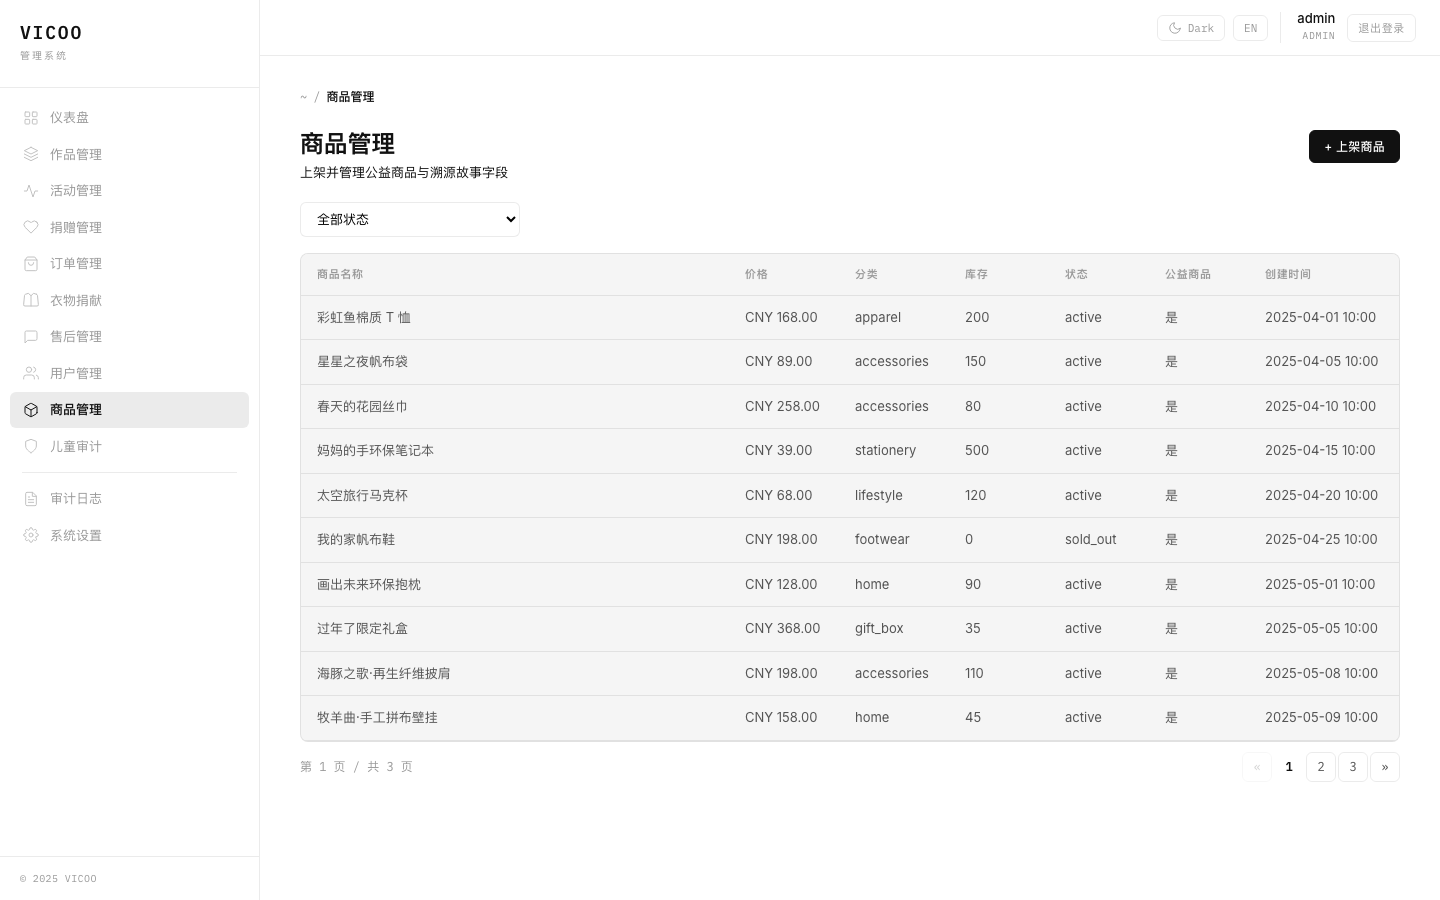
\includegraphics[width=0.94\linewidth]{user-manual-figures/u3-admin-products.png}\caption*{Figure U3: Admin console --- Products (\texttt{/admin/products}).}\end{figure}%
}{\placeholder{Generate \texttt{user-manual-figures/u3-admin-products.png} (start \texttt{admin} dev server first).}}

\subsection{Typical Flow 3: Supply-Chain Journey Data}
\textbf{Steps:}
\begin{enumerate}[leftmargin=2.2em]
    \item Confirm how your environment loads timeline/globe data (database seed, migration, or API tooling).
    \item After changing journey rows, reload \texttt{/impact/shop/:id} and verify node count, ordering, and stage labels.
\end{enumerate}

\textbf{Expected result:}
Consumer timeline and globe match the back-end source of truth. If no admin UI exists for nodes in your build, document the maintenance path so testers do not expect on-screen node editors.

\subsection{Typical Flow 4: Reviewing AI-Assisted or Third-Party Copy}
\textbf{Steps:}
\begin{enumerate}[leftmargin=2.2em]
    \item Collect AI-generated drafts separately from production fields.
    \item Compare drafts against verified product facts, campaign legal text, and child-safety policies where applicable.
    \item Paste only vetted text into admin or CMS fields; keep exaggeration and unverifiable claims out of live copy.
\end{enumerate}

\textbf{Expected result:}
Published strings align with structured data; no fabricated certificates, geographies, or donation outcomes.

\subsection{Common Questions for Staff}
\textbf{Question 1: Why are admin changes not visible on the consumer site?}\\
Answer: Confirm the save API succeeded, hard-refresh the consumer app, and verify you are viewing the correct product ID and shop (\texttt{/shop} vs \texttt{/impact/shop}).

\textbf{Question 2: Where do I edit globe nodes?}\\
Answer: Not on the current Products form; use the data path your team documents (seed scripts, SQL, or future tooling).

\textbf{Question 3: Can AI drafts go live without review?}\\
Answer: No. Treat AI output as provisional; human approval is mandatory before public display.

\section{Partner / Supply Chain Information Provider Guide (Roadmap)}
\subsection{Current Status}
The production codebase does \textbf{not} ship a partner-facing portal or partner role for self-service uploads. Partner organisation names may appear as attributes on consumer timeline stages. Treat the following as a \emph{design target} for future iterations or course narrative, not as mandatory test cases unless you implement them.

\subsection{Target Workflow (Future)}
\begin{enumerate}[leftmargin=2.2em]
    \item Authenticate partners into a restricted workspace.
    \item Scope edits to assigned SKUs or stages.
    \item Submit evidence; route submissions through staff review before publication.
\end{enumerate}

\textbf{Expected result (when built):} least privilege, pending-review states, and audit trails comparable to existing admin patterns.

\section{Testing Suggestions and Acceptance Focus}
\begin{enumerate}[leftmargin=2.2em]
    \item \textbf{Dual shop correctness}: URLs, product flags, and merchandising differ between \texttt{/shop} and \texttt{/impact/shop}.
    \item \textbf{Globe preconditions}: only eligible impact URLs with data show the immersive globe.
    \item \textbf{Data synchronisation}: admin product fields match consumer rendering; timeline data matches API JSON.
    \item \textbf{Transactional paths}: cart, checkout, and order detail for smoke coverage.
    \item \textbf{Auth-gated features}: review submission requires login; errors are understandable.
    \item \textbf{AI discipline}: assistant answers and marketing copy are curated before demos.
    \item \textbf{Accessibility baseline}: keyboard focus and readable contrast on long editorial pages.
\end{enumerate}

\section{Closing Remarks}
This guide ties each role to observable routes and admin modules in the \projectname{} repository. Keeping terminology aligned with the code (\texttt{/impact/shop}, impact flags, admin sidebar) reduces false failures during evaluation and demonstrates engineering maturity beyond a static mock-up.

\section*{References}
\begin{enumerate}[leftmargin=2.2em]
    \item React Team. \emph{React v18 Documentation}. 2024. Available at: \url{https://react.dev/}.
    \item Vite Team. \emph{Vite Guide}. 2025. Available at: \url{https://vite.dev/guide/}.
    \item Three.js Contributors. \emph{Three.js Manual}. 2025. Available at: \url{https://threejs.org/manual/}.
    \item FastAPI Contributors. \emph{FastAPI Documentation}. 2025. Available at: \url{https://fastapi.tiangolo.com/}.
    \item W3C Web Accessibility Initiative. \emph{Web Content Accessibility Guidelines (WCAG) 2.2}. W3C Recommendation, 2023. Available at: \url{https://www.w3.org/TR/WCAG22/}.
\end{enumerate}

\end{document}
